
%
% d3 Tutorial CISNET Programmers Breakout November 2, 2011
%
%  Author: Ben Racine
%  Date:   November 2nd 2011
%
%  Compile this document with:
%    pdflatex <filename>.tex


\documentclass[notes]{beamer}
%\documentclass{beamer}  


\mode<presentation>
{
% \setbeamertemplate{background canvas}[vertical shading][bottom=red!10,top=blue!10]
%
  \usetheme{Warsaw}
  \usecolortheme{default}
  \usefonttheme[onlysmall]{structurebold}
}


\setbeamercolor{math text}{fg=red!50!black}
\setbeamercolor{normal text in math text}{parent=math text}

\usepackage{pgf,pgfarrows,pgfnodes,pgfautomata}
\usepackage{amsmath,amssymb}
\usepackage{lmodern}
\usepackage[latin1]{inputenc}
\usepackage{colortbl}
\usepackage{fancybox, stmaryrd}
\usepackage[english]{babel}

\usepackage{lmodern}
\usepackage[T1]{fontenc} 

\usepackage{times}
\setbeamercovered{dynamic}



\title{Period Three Implies Hardcore Chaos}
\author[Curtius]{
Kit Curtius \inst{1}
}
\institute[]{
\inst{1}
University of Washington, Applied Mathematics, USA
}
 
\date[AMath 2011]{AMATH 575 Final Presentation\\
June 4, 2011}

\begin{document}

\frame{\titlepage}

\part<presentation>{Main Talk}

\begin{frame}
  \frametitle{Outline}
%  \tableofcontents[part=1,pausesections]
   %\tableofcontents[pausesections] 
    \tableofcontents
\end{frame}


\section[History]{History}
\subsection[Sarkovskii's Theorem]{Sarkovskii's Theorem}

%\begin{frame}
% \frametitle{Oleksandr Mikolaiovich Sarkovskii}
%{\footnotesize
%\begin{columns}
%\column{ .25\textwidth}
%\vskip .2cm
%
\includegraphics[height =1.5 in]{Sharkovsky.jpg}
%\column{.65\textwidth}
%\vskip -.5cm
%\begin{itemize}
%\item Ukrainian mathematician born December 7, 1936. 
%\item Paper published in \emph{Ukrainian Mathematical Journal} in 1964 (Vol. 16, pp 61-71) entitled \textbf{Coexistence of Cycles of a Continuous Map of a Line into Itself}.
%\item \emph{Sarkovskii ordering of the natural numbers:}\\ $ 3 \rhd 5 \rhd 7 \rhd \dots \rhd2\cdot 3 \rhd 2\cdot 5\rhd \dots$\\
%$2^2\cdot 3 \rhd 2^2 \cdot 5 \rhd \dots \rhd 2^3\cdot 3 \rhd 2^3 \cdot 5 \rhd \dots \rhd 2^ 3 \rhd 2^2 \rhd  2 \rhd 1$
%\end{itemize}
%\end{columns}
%}
%\begin{block}{ Sarkovskii's Theorem}
%Suppose $ F: \mathbb{R} \longrightarrow\mathbb{R}$ is a continuous function with periodic point of period $k$ ( $\exists \, x $ s.t. $F^k(x) = x$ and $F^n(x)\neq x$ for $1 \leq n < k$).
%Then if $k \rhd l$ in the Sarkovskii ordering, then $F$ also has a periodic point of period $l$. 
%\end{block}
%
%\end{frame}


%\begin{frame}
%\frametitle{Implications of Sarkovskii's Theorem}
%\begin{itemize}
%\item The only assumption is that $F$ is a continuous, one-dimensional map.
%\item If $F$ has a periodic point whose period is not a power of two, it necessarily has infinitely many periodic points.
%\item Conversely, if $F$ has only finitely many periodic points, then they all necessarily have periods which are powers of 2 (period-doubling route to chaos)
%\item The "greatest" period in the Sarkovskii ordering is 3, thus the Period Three Theorem is simply a corollary to Sarkovskii's.
%\end{itemize}
%\end{frame}
%
%\subsection[Period 3 Implies Chaos]{Tien-Yien Li and James A. Yorke }
%\begin{frame}
%\frametitle{Tien-Yien Li and James A. Yorke}
%{\footnotesize
%\begin{columns}
%\column{ .25\textwidth}
%\vskip .2cm
%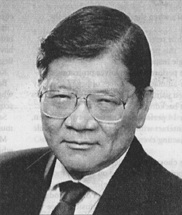
\includegraphics[height =1.3 in]{li_t.jpg}
%\column{.65\textwidth}
%\vskip -.5cm
%\begin{itemize}
%\item Paper published in \emph{The American Mathematical Monthly} in 1975 (Vol. 82, \\pp 985-992) entitled \textbf{Period Three Implies Chaos}.
%\item First appearance of the word "chaos" in scientific literature.
%\end{itemize}
%\end{columns}
%
%\begin{columns}
%
%\column{.65\textwidth}
%\vskip -.5cm
%\begin{itemize}
%\item Some time after the publication, Yorke attended a conference in East Berlin, during which Sarkovskii approached 
%him and conveyed that he had proven his results a decade earlier.
%\end{itemize}
%\column{ .25\textwidth}
%%\vskip .2cm
%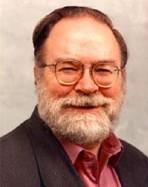
\includegraphics[height =1.3in]{yorke1.jpg}
%\end{columns}
%}
%
%\end{frame}
%
%
\section[Period 3 Proof ]{Period 3 Implies Chaos Theorem}
\subsection[Theorem and Observations]{Period 3 Proof Observations}


\begin{frame}
\frametitle{Period 3 Implies Chaos Theorem}
\begin{block} {Theorem}
Let  $ F: \mathbb{R} \longrightarrow\mathbb{R}$ be a continuous function with periodic point of period three.  Then $F$ has periodic points of all other periods. 
\end{block}

\begin{itemize}
\item \underline{Observation 1:}
 \begin{itemize}
 {\footnotesize 
 \item Suppose $I =[a,b]$ and $J =[c,d]$ are closed intervals and $I \subset J$. If $F(I) \supset J$, 
then $F$ has a fixed point in $I$.
 }
 \end{itemize}
 \item \underline {Observation 2:}
  \begin{itemize}
 {\footnotesize 
 \item Suppose $I$ and $J$ are two closed intervals and $F(I) 
\supset J$. Then there is a closed subinterval $ K \subset I$ such that $F(K) = J$. 
 }
 \end{itemize}
 \item \bf{WARNING:} This proof is set intensive, bear with me!
\end{itemize}

\end{frame}
%
%
%
%
%\begin{frame}
%\frametitle{Picture Proof of Observation 1}
%%\vspace {- .5cm} 
%\begin{columns}
%
%\column{.45\textwidth}
%\begin{itemize}
%\item \underline{Observation 1:}\\
% {\footnotesize 
% Suppose $I =[a,b]$ and $J =[c,d]$ are closed intervals and $I \subset J$. If $F(I) \supset J$, 
%then $F$ has a fixed point in $I$.
%\begin{itemize}
%\item Follows from the Intermediate Value Theorem.
%\item Since $I \subset J$, the graph of $F$ must cross the diagonal
% 
%\end{itemize}
% }
%
% \end{itemize}
%
% \column{.65\textwidth}
%
% 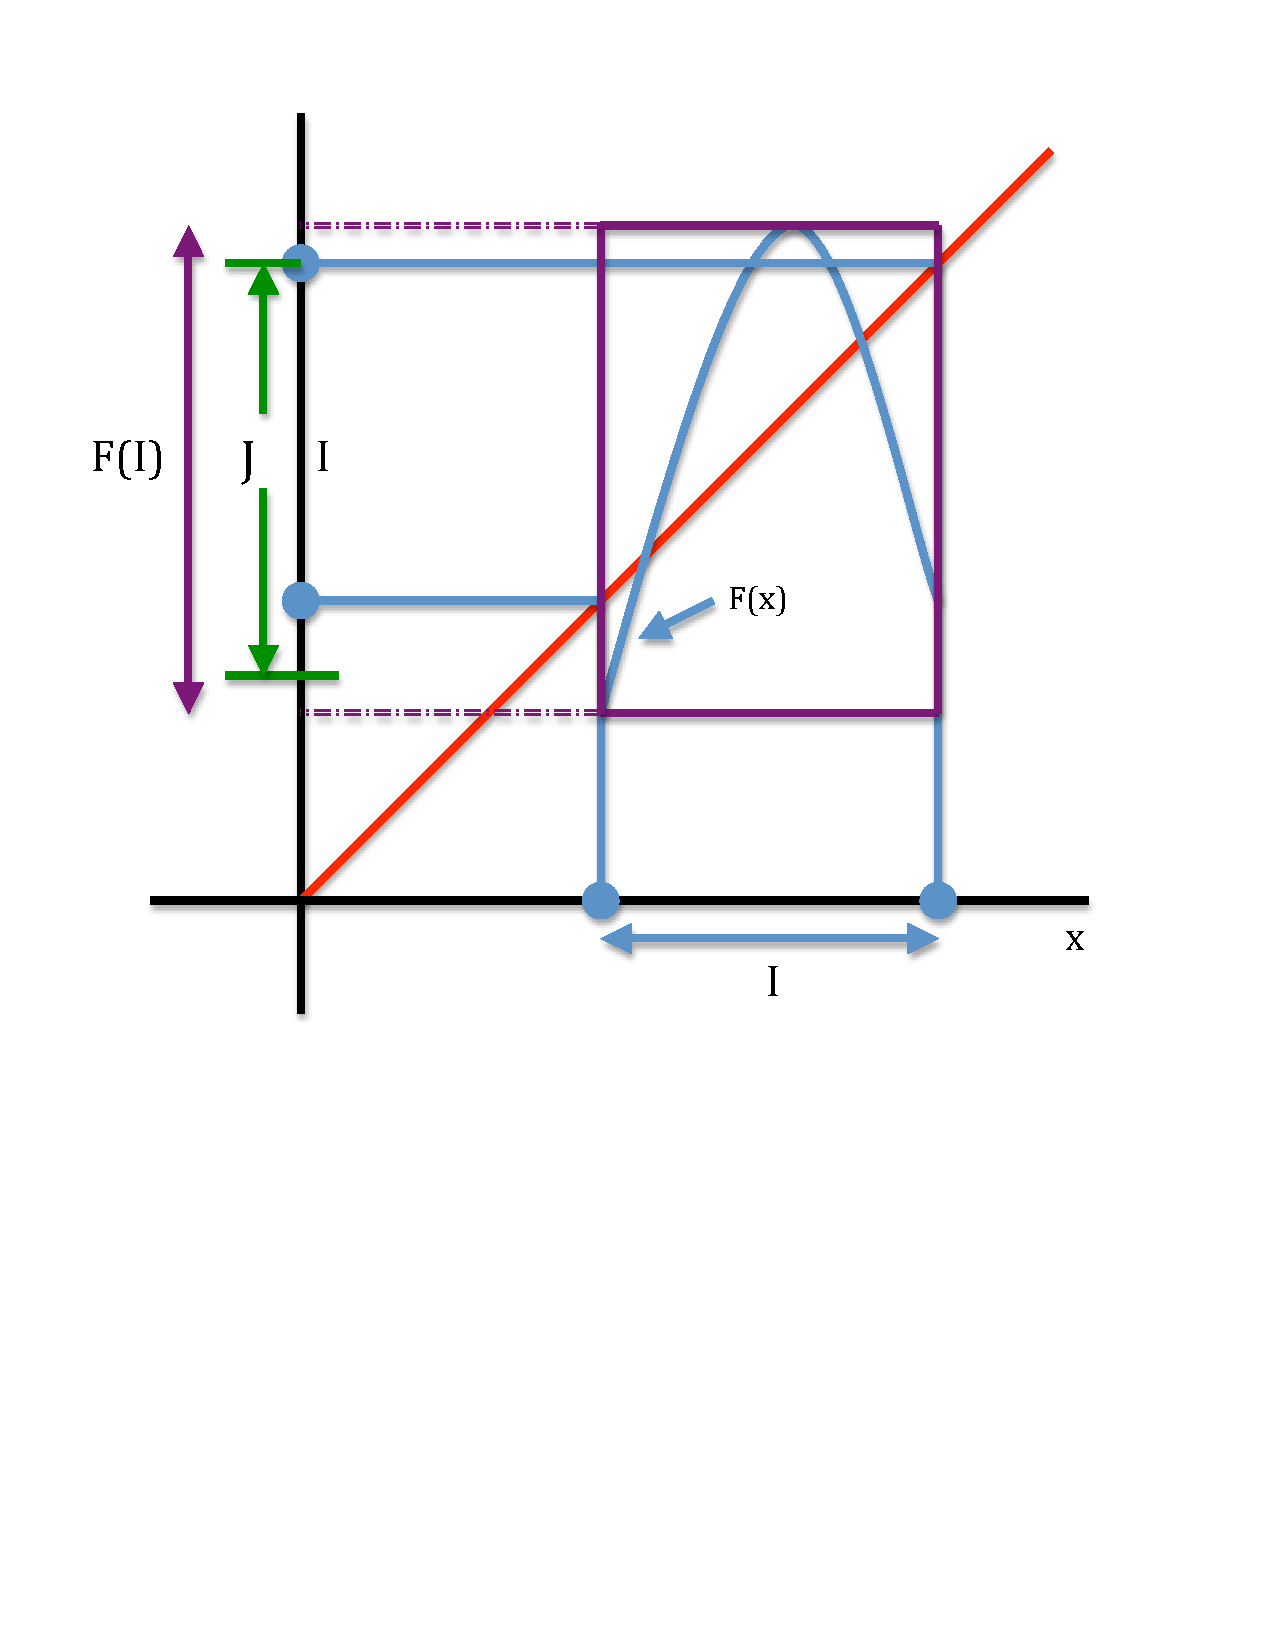
\includegraphics[height =2.5in]{observ1.pdf}
% \end{columns}
%\end{frame}
%
%
%
%
%\begin{frame}
%\frametitle{Picture Proof of Observation 2}
%\begin{columns}
%\column{.5\textwidth}
%\begin{itemize}
%\item \underline{Observation 2:}\\
%
% {\footnotesize 
% Suppose $I$ and $J$ are two closed intervals and $F(I) 
%\supset J$. Then there is a closed subinterval $ K \subset I$ such that $F(K) = J$. 
% }
%
% \end{itemize}
% \column{.65\textwidth}
%
% 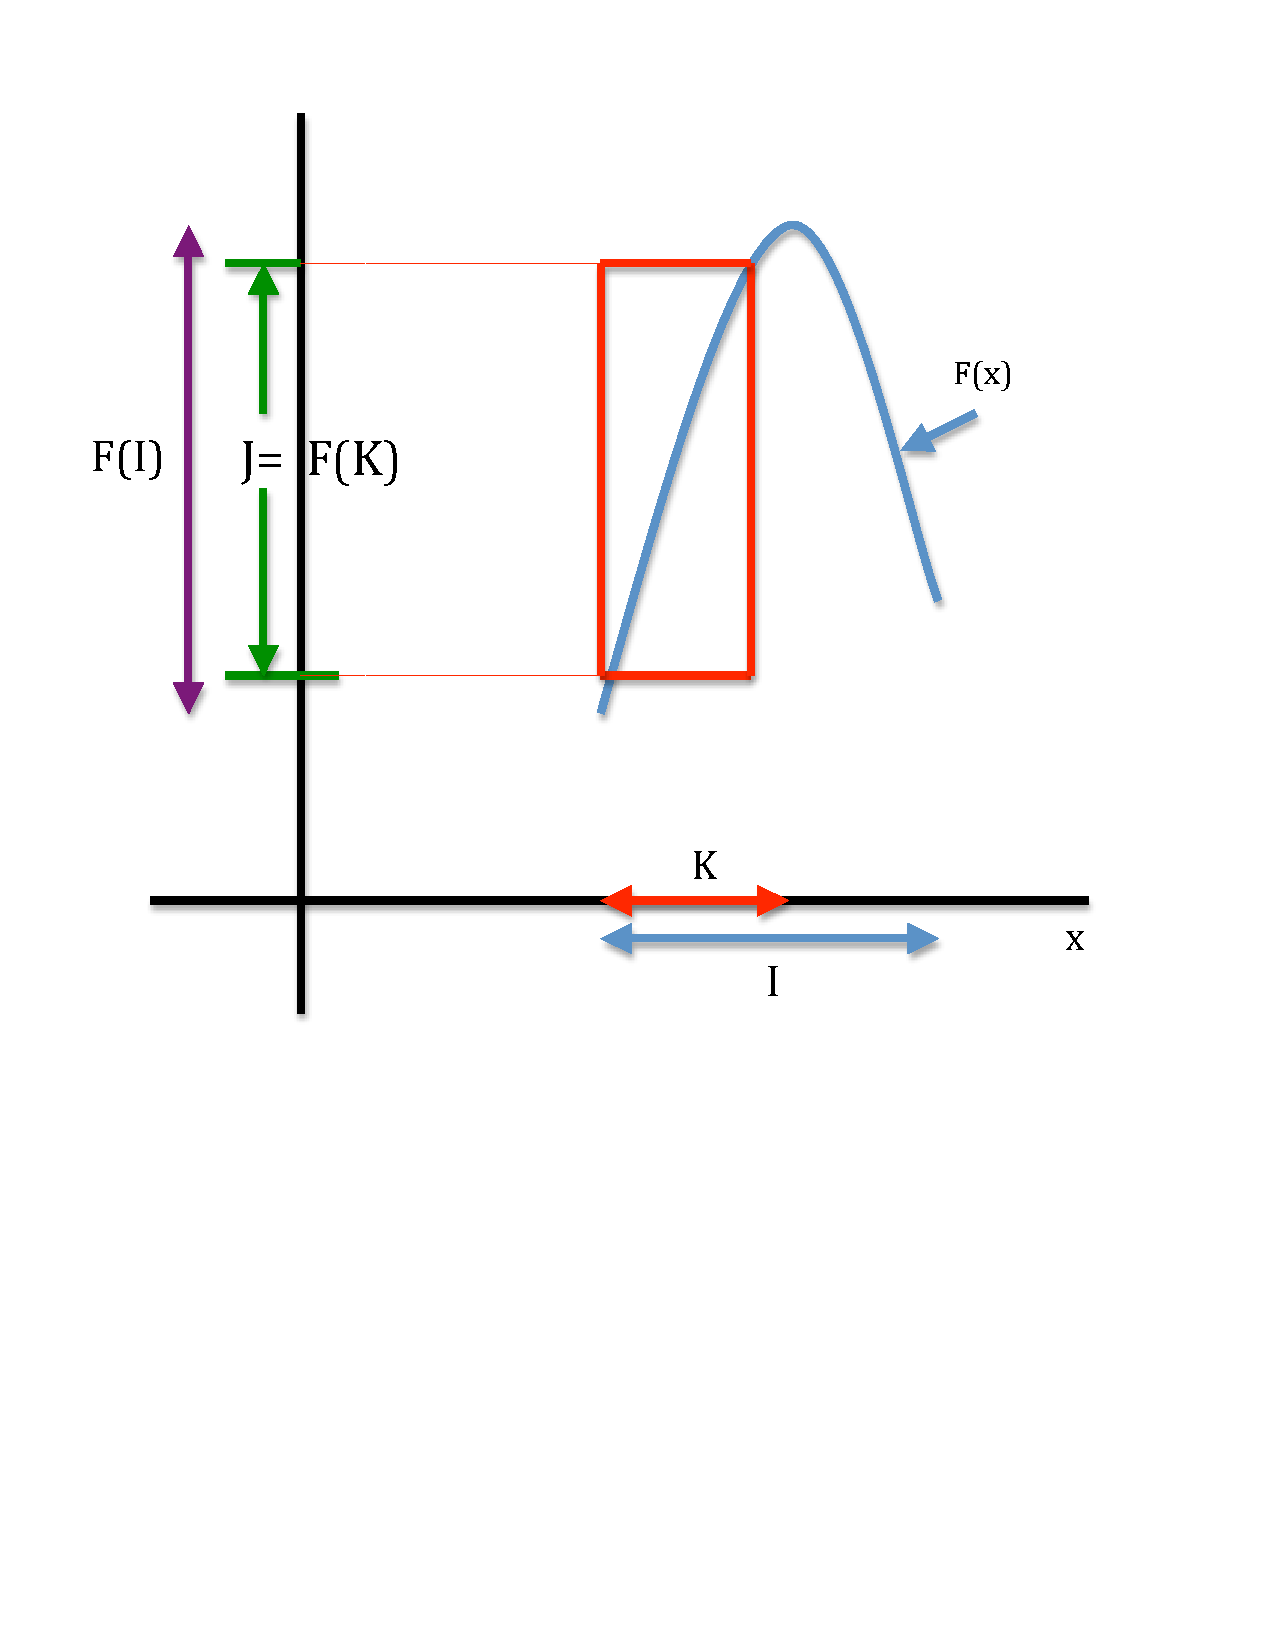
\includegraphics[height =2.5in]{observ2.pdf}
% \end{columns}
%\end{frame}
%
%
%\subsection[Proof Setup and Steps]{Proof of Period 3 Theorem}
%\begin{frame}
%\frametitle{First Steps and Diagram}
%
%{\scriptsize
%\vskip -.3cm
%\begin{itemize}
%\item Let $a,b,c \in \mathbb{R}$. Suppose $F(a) = b, F(b) = c, F(c)=a$ \\
%$ \Rightarrow a\rightarrow b \rightarrow c \rightarrow a \,\,\,\,\,\, $  $F$ has a period three-cycle .
%
% \item We will assume $a$ is the leftmost point on the real line.  Then we will assume $a < b < c$.  The only other case $a < c < b$ is handled similarly.
%\end{itemize}
%}
%
%\begin{columns}
%\column{.5\textwidth}
% {\footnotesize 
%\begin{itemize}
%\item Let $I_0 = [a,b]$ and $I_1=[b,c]$\\
% By continuity of $F$:\\
% \begin{enumerate}
% \item
%$F(a) = b, F(b) = c$\\
%$\Rightarrow$ \doublebox{$ I_1 \subset F(I_0)$}\\
%\item
%$F(b) =c, F(c) = a $\\
% \doublebox{ $F(I_1) \supset [a,c] = I_0 \cup I_1$}
%\end{enumerate}
%\item First we will construct periods 1 and 2 and then periods $n > 3$
% 
%
% \end{itemize}
% }
% \column{.65\textwidth}
%
% 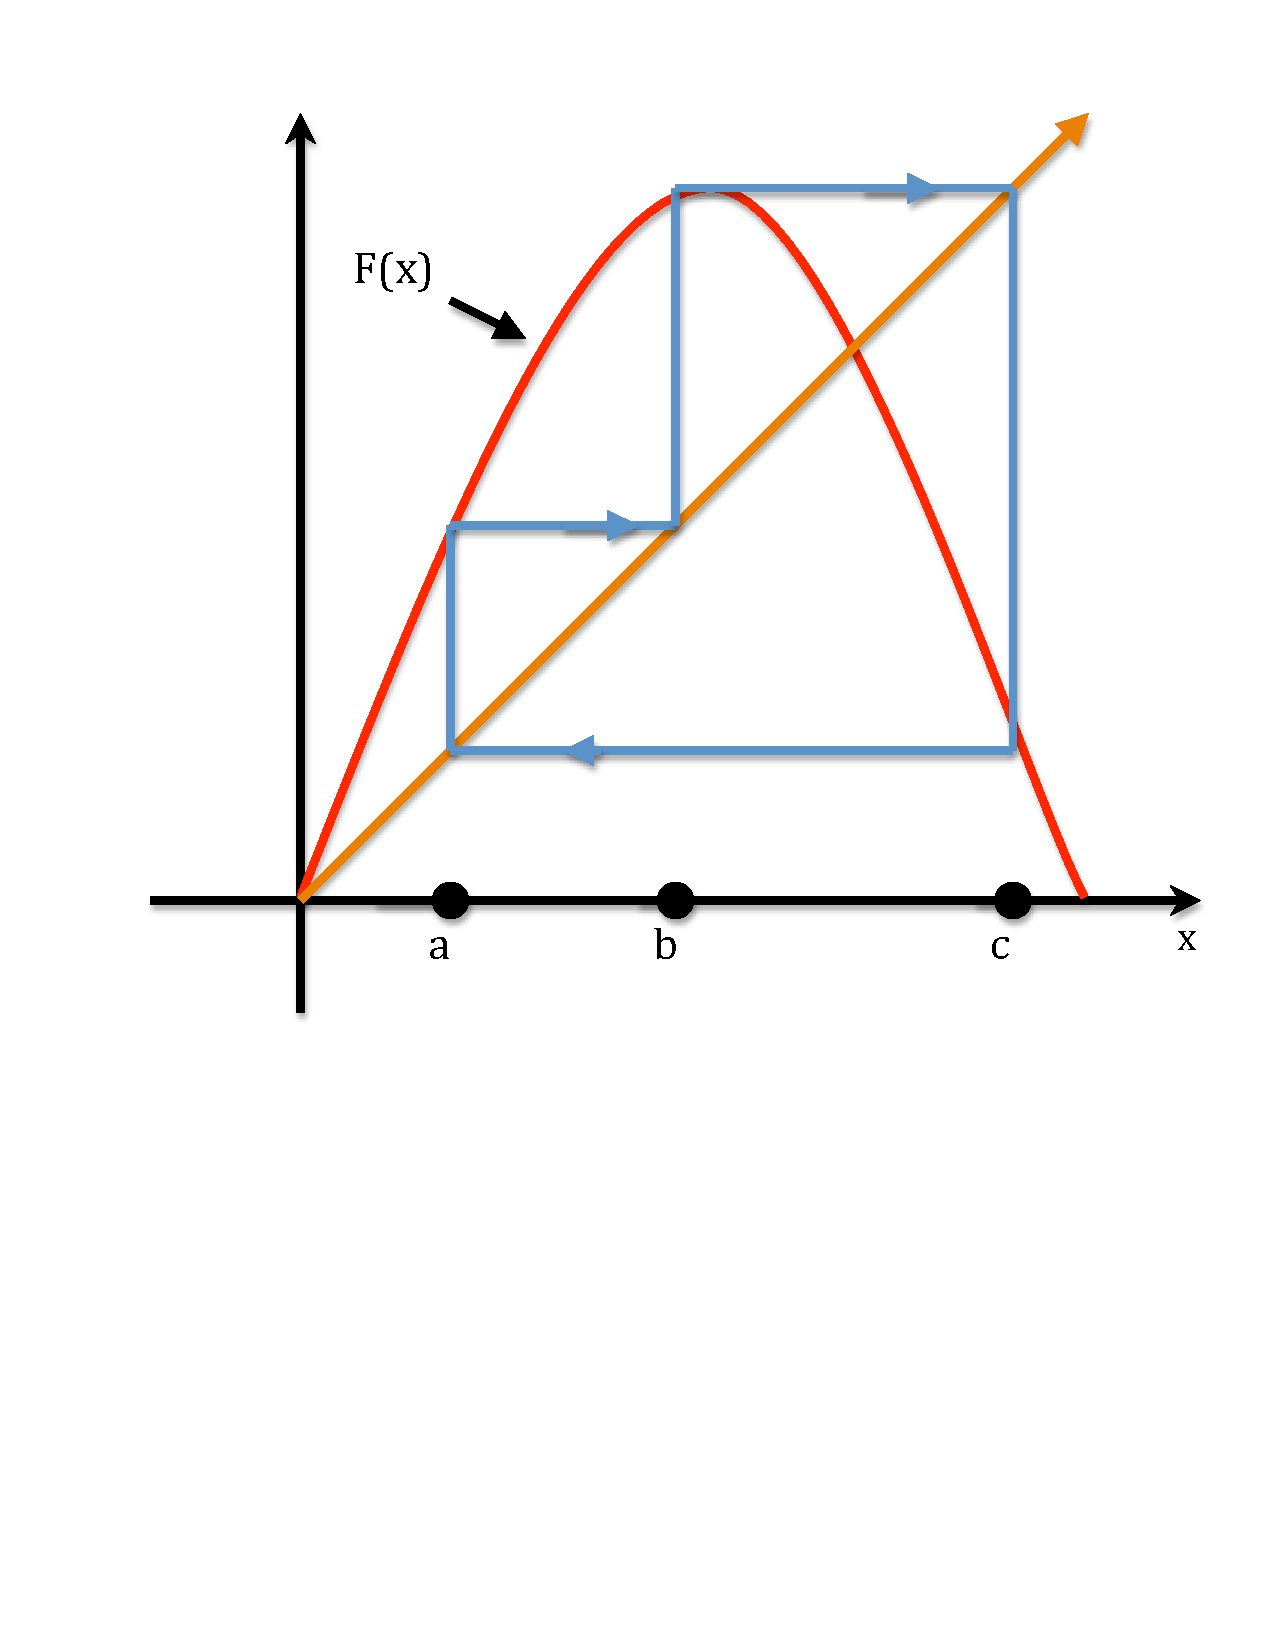
\includegraphics[height =2.2in]{period3fexample.pdf}
% \end{columns}
%\end{frame}
%
%
%\begin{frame}
%\frametitle{Cases for n=1 and n=2}
%\begin{block}{Existence of point with period 1}
%We have just shown that $ I_0 \cup I_1\subset F(I_1) $ thus $I_1 \subset F(I_1)$\\
%Clearly $I_1 \subset I_1$, always, therefore by Observation 1, we know there exists a fixed point of $F$ in $I_1$.\\
%$\Rightarrow \exists \,x_1  \in I_1$ s.t. $ F(x_1) = x_1$ so $x_1$  has period 1.
%
%\end{block}
%
%\begin{block}{Existence of point with period 2}
%Likewise, we showed that $ I_1 \subset F(I_0)$ and we know $I_0 \subset F(I_1)$ since  $ I_0 \cup I_1\subset F(I_1) $.  Therefore $ I_0\subset F^2(I_0) $.\\
%Again $I_0 \subset I_0$ so by Observation 1, we know there exists a fixed point $x_2$ of $F^2$ in $I_0$ and from diagram of $F$ we can see that this is indeed an orbit
%of period 2 since $F(x_2) \in I_1$ (more to come on this later).
%\end{block}
%
%\end{frame}
%
%\begin{frame}
%\frametitle{Periods of length n > 3}
%{\footnotesize
%\begin{itemize}
%\leftskip -1cm
%\item To find a point for each period $n >3$ we will invoke Observation 2  $n-1$ times and Observation 1 on the last step.
%\item Since $F(I_1) \supset I_1$, by Observation 2,  there is a subinterval $A_1 \subset I_1$ s.t. $F(A_1) = I_1$
%\item Again invoking Observation 2, since $F(A_1) \supset A_1$, we can find a closed subinterval $A_2 \subset A_1$ s.t.  $F(A_2) = A_1$\\
%Note that by construction,  we now have sets $A_2 \subset A_1 \subset I_1$. 
%\item Continue this process $n-2$ times. By now we have produced a collection of closed nested intervals $A_i$ , $1 \leq i \leq n-2$ s.t.
%\begin{center}
%$A_{n-2} \subset A_{n-3} \subset \dots \subset A_2 \subset A_1 \subset I_1$
%\end{center}
%where $F(A_i)  = A_{i-1}$ and $F(A_1) = I_1$.  Note that $A_{n-2} \subset I_1$ and $F^{n-2}(A_{n-2}) = I_1$
%\end{itemize}
%
%}
%\end{frame}
%
%\begin{frame}
%\frametitle{Periods of length n > 3 (cont.)}
%{\footnotesize
%\begin{itemize}
%\leftskip -1cm
%\item Since $I_0 \subset F(I_1)$, equivalently $I_0 \subset F^{n-1}(A_{n-2})$, there exists a closed subinterval (you guessed it, by Obs. 2) $A_{n-1} \subset A_{n-2}$ s.t. $F^{n-1}(A_{n-1}) = I_0$.  
%\item Lastly, since $I_1 \subset F( I_0)$ we have $I_1\subset F^n(A_{n-1})$.  Thus since $A_{n-1} \subset I_1$ by construction, then we invoke Observation 1
%to conclude that there exists a point $x_n \in A_{n-1}$ s.t. $F^n(x_n) = x_n$. 
%
%%
%%\item Since $A_{n-2} \subset I_1 \subset F(I_0)$, there is a closed subinterval (you guessed it, Obs. 2) $A_{n-1} \subset I_0$ s.t. $F(A_{n-1}) = A_{n-2}$
%%\item Lastly, since $ F(I_1) \supset I_0 \supset A_{n-1}$, there is a closed subinterval $ A_n \subset I_1$ s.t. $F(A_n) = A_{n-1}$.  Therefore we have expanded
%%our sequence to:
%%\begin{center}
%%$A_n \subset A_{n-1} \subset A_{n-2} \subset A_{n-3} \subset \dots \subset A_2 \subset A_1 \subset I_1$
%%\end{center}
%%Where $ F^n(A_n) = I_1$ and $A_n \subset I_1$.  Thus we may invoke Observation 1 to conclude that there exists a point $x_n \in A_n$ s.t. $F^n(x_n) = x_n$.  
%\item \underline{Claim:} $n$ is the LEAST period of $x_n$.  \\
%Note:   Suppose $F^{n-1}(x_n)$ lies on the boundary of $I_0$.  Then $F^{n-1}(x_n) = a$ or $b$ (on the period 3 orbit, started from $b$ or $c$) so $n=2$ or $n=3$ necessarily. This contradicts our assumption that $n >3$, we have already dealt with these cases.  \\
%Thus $F^{n-1}(x_n)$ lies on the interior of $I_0$.  We know the first $n-2$ iterations of $x_n$ lie in $I_1$ while $F^{n-1}(x_n) \in I_0$ and $F^n(x_n) = x_n \in I_1$ again.  If $x_n$ had period less than $n$ then it would never leave $I_1$.  Thus $x_n$ cannot have period less than $n$ \\
%\centering
%$\Rightarrow$ \shadowbox{$ x_n$ is a periodic point of $F$ with period $n$}  $\,\,\,\, \boxempty $
%
%\end{itemize}
%}
%
%\end{frame}
%
%\begin{frame}
%
%
%\frametitle{Diagram of nested interval mappings}
%\begin{columns}
%\column{.4\textwidth}
%\begin{itemize}
%{\scriptsize
%\item Studying how certain sequences of sets are mapped into or onto each other is common in dynamical systems: ex. Sarkovskii's proof and Smale's horseshoe.
%}
%\end{itemize}
%\column{.8\textwidth}
% 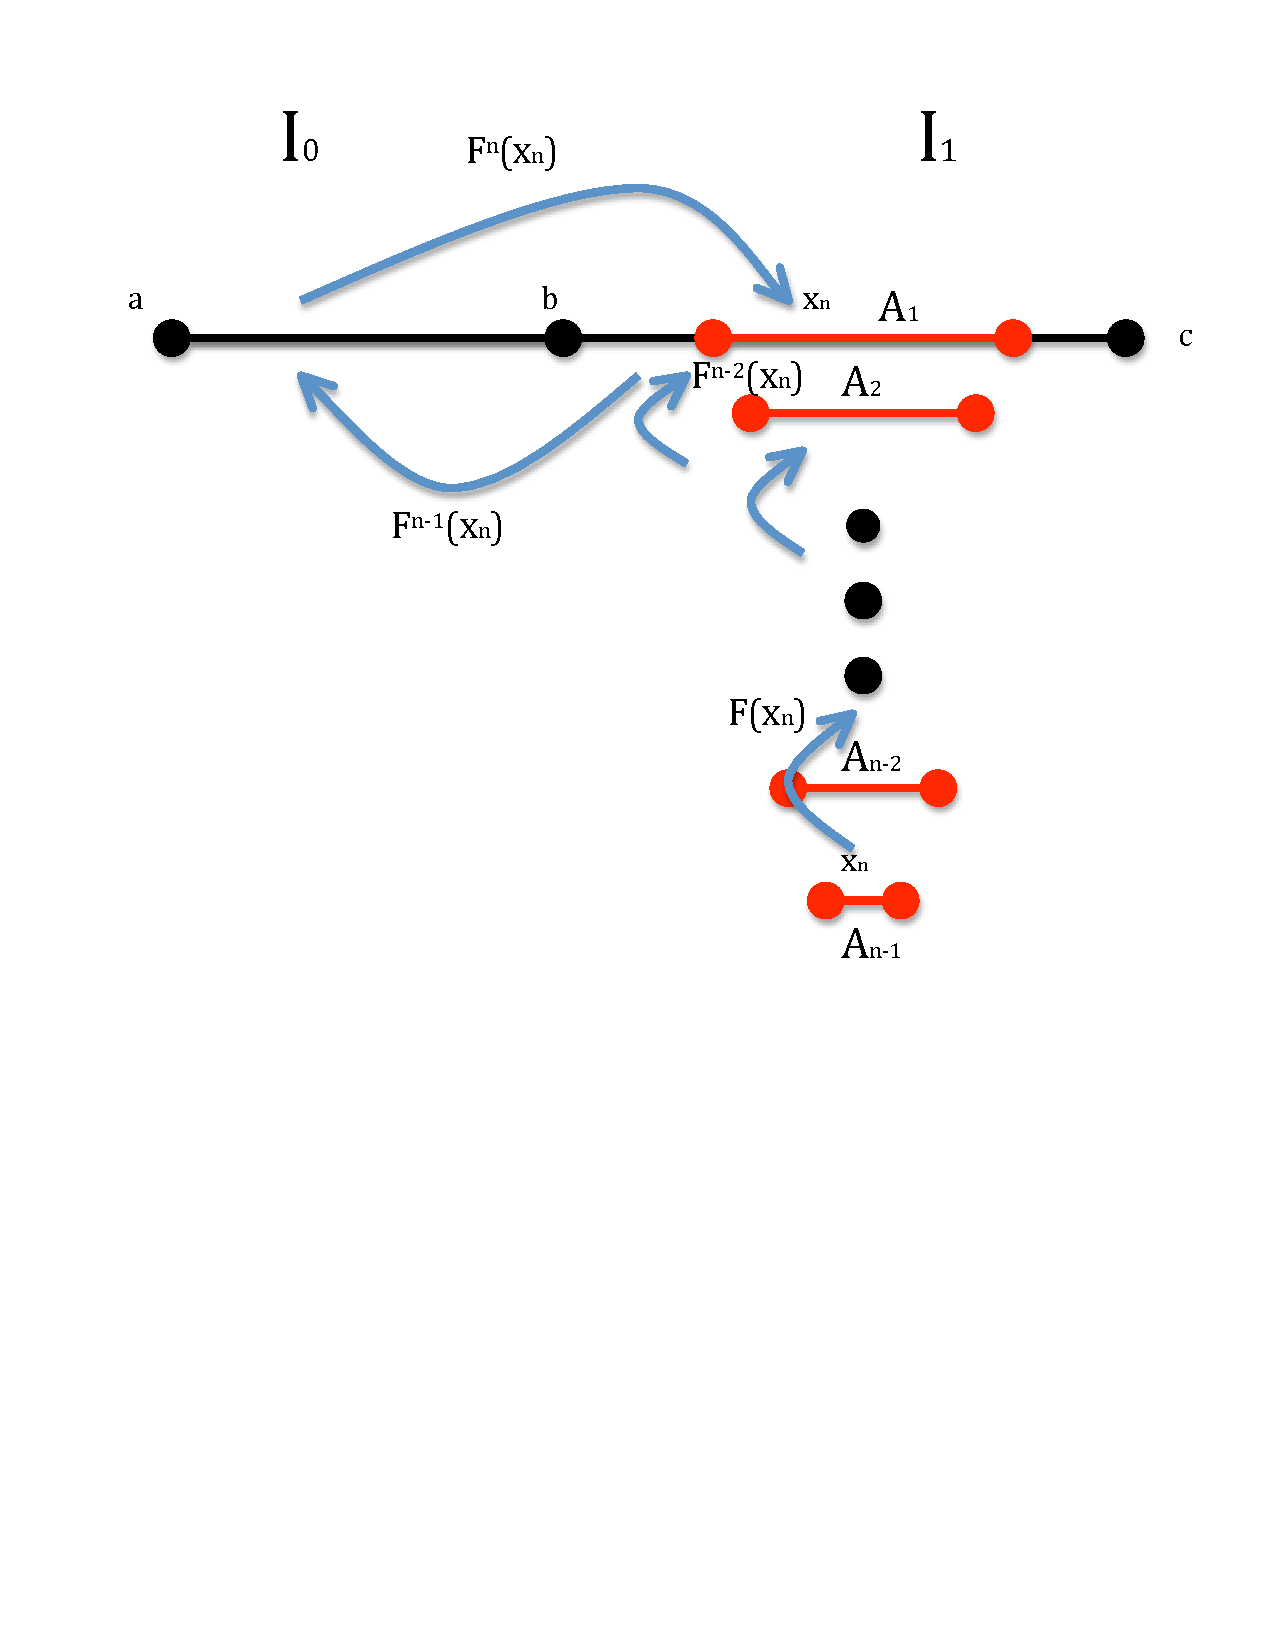
\includegraphics[height =3in]{period3nest.pdf}
%\end{columns}
%\end{frame}
%
%
%
%\subsection[Converse Example]{Converse of Sarkovskii's Theorem}
%\begin{frame}
%\frametitle{Converse is True!}
%
%\begin{block}{ Converse of Sarkovskii's Theorem}
%For any natural number $n$, there exists a continuous function $ F: \mathbb{R} \longrightarrow\mathbb{R}$ such that if $k \rhd n$ in the Sarkovskii ordering, $F$ has a periodic point of period $n$ but none of period $k$ 
%\end{block}
%\begin{itemize}
%\item Of course, this is again a  generalization to the same converse result for the Period Three Theorem since 3 precedes all numbers in the Sarkovskii ordering.
%\item We will show the example of a function $F$ with a period 5 point but no points of period 3 from Li and Yorke's paper.
%\end{itemize}
%\end{frame}
%
%\begin{frame}
%\frametitle{Converse Example}
%\begin{columns}
%\column{.5\textwidth}
%\begin{itemize}
%\item Consider the piecewise linear map $F : [1,5] \longrightarrow [1,5]$ where
%\[1 \rightarrow 3 \rightarrow 4 \rightarrow 2 \rightarrow 5 \rightarrow 1\]
%\item That is, $F^5(1) = 1$ :\\ $F$ has a 5-cycle.
%
% {\footnotesize 
%\item  We claim $F$ has no 3-cycle 
% }
%
% \end{itemize}
% \column{.65\textwidth}
%
% 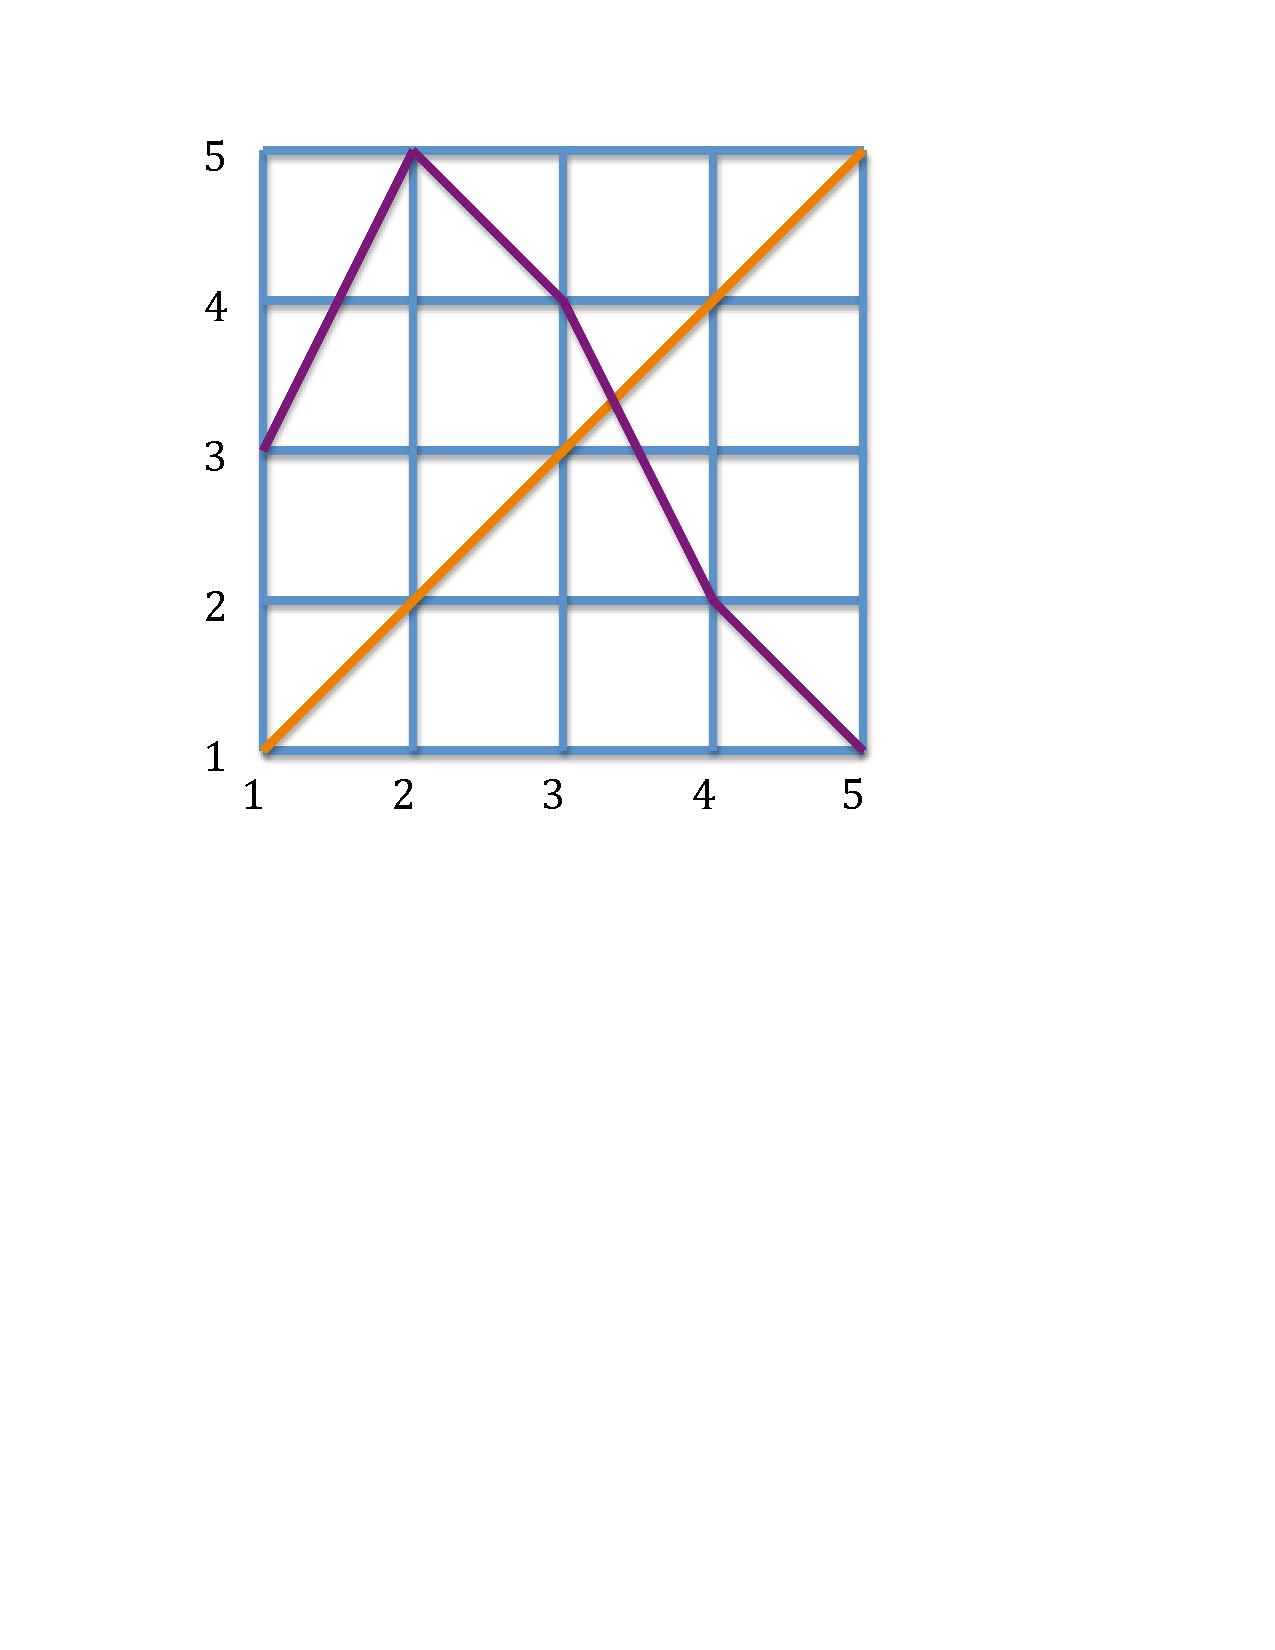
\includegraphics[height =2.9in]{sarkovskiiconv.pdf}
% \end{columns}
%
%\end{frame}
%
%
%\begin{frame}
%\frametitle{Converse Example (cont.)}
%\begin{columns}
% \column{.5\textwidth}
%
% 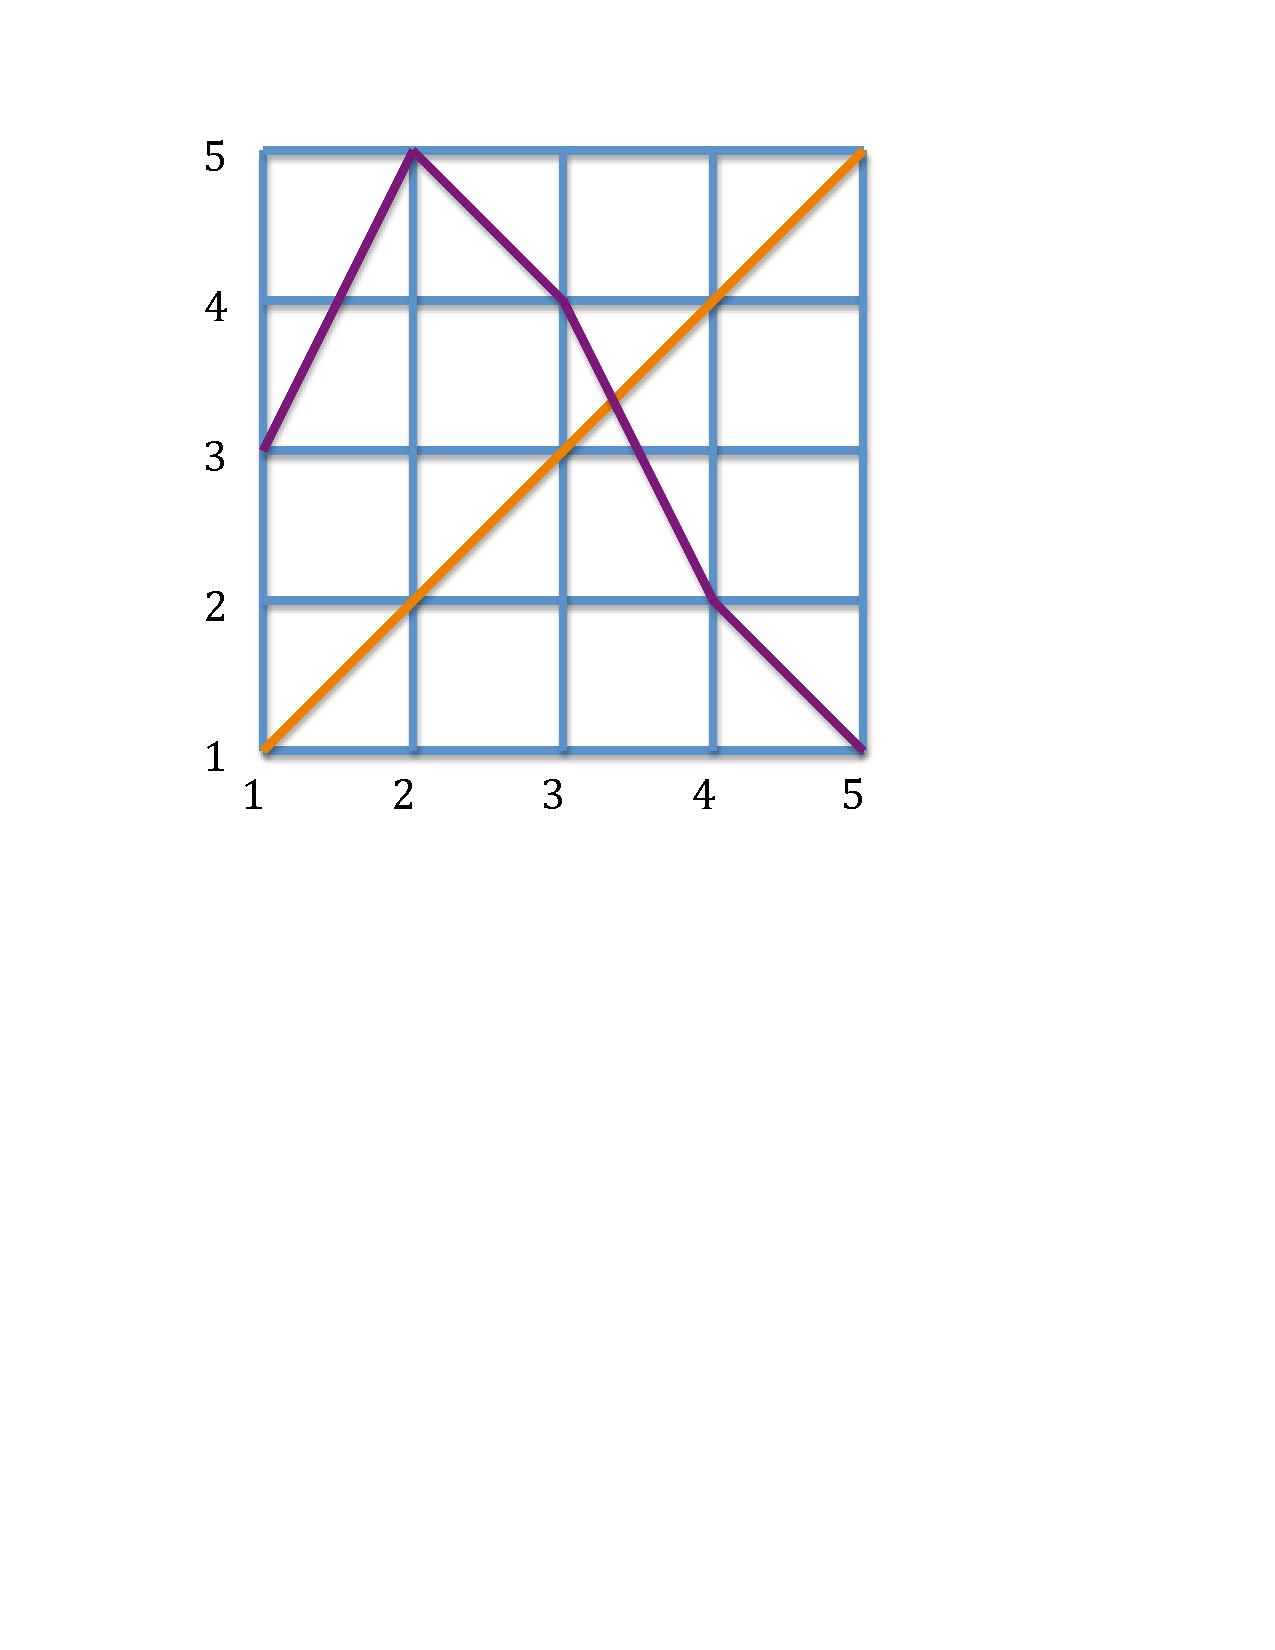
\includegraphics[height =2.5in]{sarkovskiiconv.pdf}
% 
%\column{.75\textwidth}
%\begin{itemize}
%{\footnotesize
%\item $F([1,2]) = [3,5], F([3,5]) = [1,4],$\\
%$ F([1,4]) = [2,5] \Rightarrow F^3([1,2]) = [2,5]$
%\item Thus the only fixed point of $F^3$ in $[1,2]$ could be \\
%2 but 2 has period 5 on the 5-cycle.
%\item Similarly  we can check $F^3$ has no fixed pts. in\\
% $[2,3]$ or $[4,5]$
%\item $F$ has a fixed pt. on $[3,4]$ and we see that
% $F([3,4]) = [2,4], F([2,4]) = [2,5],$\\
%$ F([2,5]) = [1,5] \Rightarrow F^3$ has a fixed pt. in $[3,4]$
%\item \underline{Claim:} This fixed pt. of $F^3$ is unique and is thus \\the fixed pt. of $F$ itself (not least period 3).
%\item $F$ is monotonically decreasing on $[3,4] \rightarrow [2,4] \rightarrow [2,5]\rightarrow [1,5]$ thus $F^3$ \\
%is monotonically decreasing also and the \\
%fixed pt. is unique $\rightarrow F$ has no 3-cycles 
%}
% \end{itemize}
%
% \end{columns}
%
%
%\end{frame}
%
%
%
%
%\section[Results]{Results and Examples}
%\subsection[Logistic Map Example]{Logistic Map}
%
%%\usebackgroundtemplate{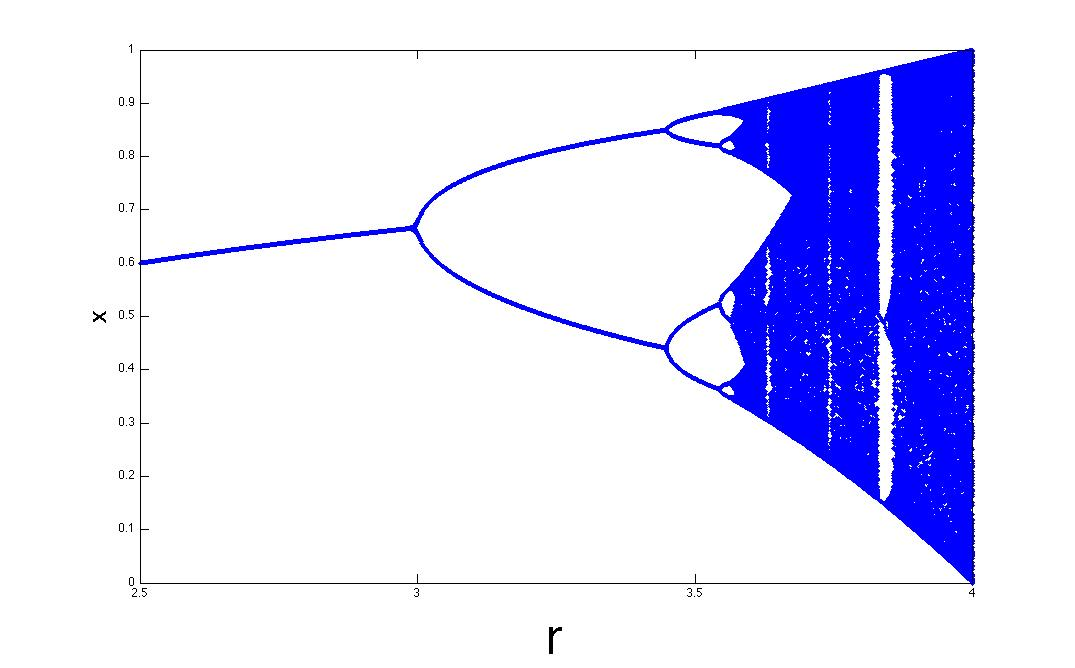
\includegraphics[height=\paperheight, width=\paperwidth]{logistic575.jpg}}
%\begin{frame}
%\frametitle{Analysis of Logistic Map}
%
%\begin{columns}
%\column{.5\textwidth}
%\begin{block}{"The snake in the mathematical grass" - Robert May}
%\begin{itemize}
%%{\scriptsize
%\item $x_{n+1} = r \,x_n (1-x_n )= F(x_n)$
%%\begin{itemize}
%\item NOTE: each $r$ value specifies a DIFFERENT $F$ where Li and Yorke's theorem holds.
%\item  Sarkovskii's results confirmed: If $F$ has only finitely many periodic points, then it necessarily
%has periods which are powers of 2.
%%\end{itemize}
%%}
% \end{itemize}
%\end{block}
% \column{.5\textwidth}
%\begin{figure}[h!]
%\centering
%\vskip -1cm
%\rightskip-2cm
% 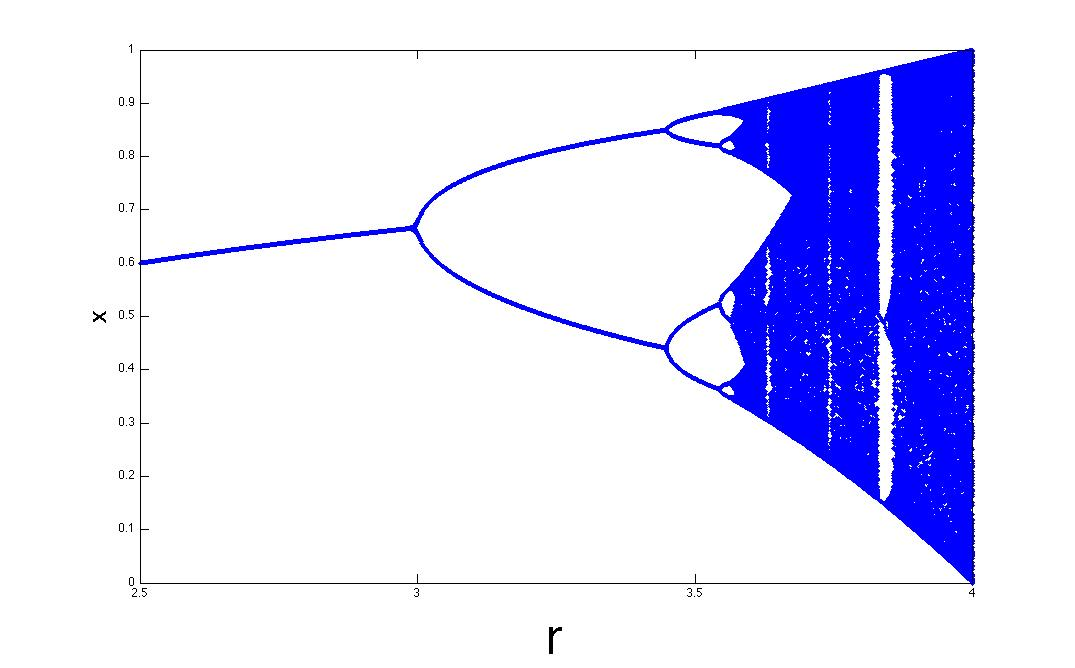
\includegraphics[height = 2.75 in, width = 2.5in]{logistic575.jpg}
%\centering
% \end{figure}
%
% \end{columns}
%
%\end{frame}
%
%
%
%\begin{frame}
%\frametitle{ Period 3 window }
%\vskip -1cm
%\leftskip -2cm
%\begin{columns}
%
% \column{.65\textwidth}
%\begin{figure}[h!]
% 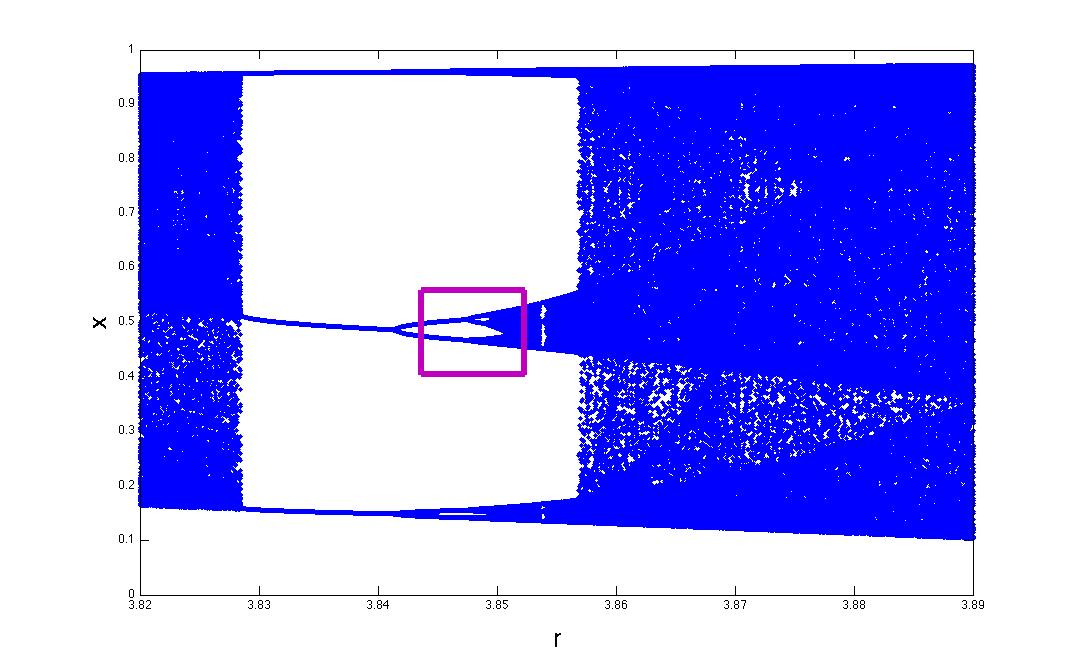
\includegraphics[height =3in]{period3-1.jpg} 
%
% \caption{ "The snake in the mathematical grass'' -Robert May} 
% \end{figure}
%\column{.5\textwidth}
%\vskip-.5cm
% 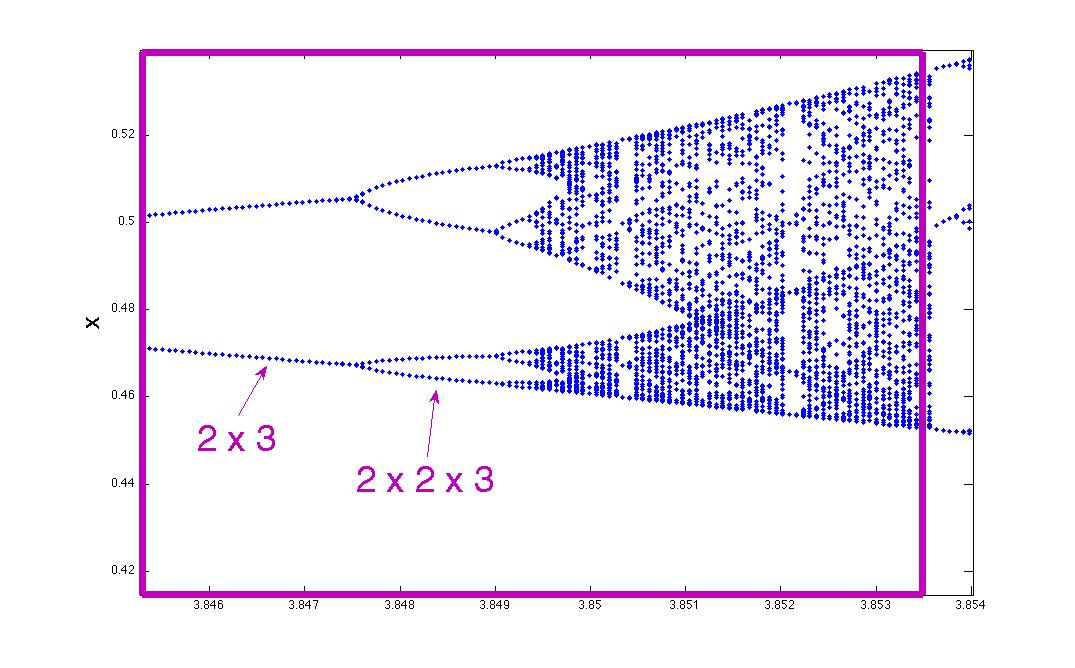
\includegraphics[height=1.5in]{period3-2.jpg}
% \vskip -.5cm
% \begin{block}{Why only period 3?}
%\begin{itemize}
%{\footnotesize
%\item When $1 + \sqrt{8} < r <  3.8415..., \,\, F$ has a 3-cycle. According to Sarkovskii's theorem, it must also have cycles of any period. 
%\item \emph{Where are these infinite period orbits?? }
%%\item Computers will plot only ATTRACTING cycles.  The period 3-cycle is the only stable period in this range of $r$ values.
%%\item Every time a new cycle is born, it is attracting, while the previous one becomes repelling. In this process, the periodic orbits are never destroyed. Rather they just become repelling. 
%%\item The set of periodic orbits steadily gets larger as $r$ increases. 
%% Fatou theorem: every attracting cycle for a polynomial or rational function attracts at least one critical point.
%
%
%}
%
%\end{itemize}
%\end{block}
%\end{columns}
%\end{frame}
%
%\begin{frame}
%\frametitle{Logistic map plot}
%\leftskip -1 cm
% 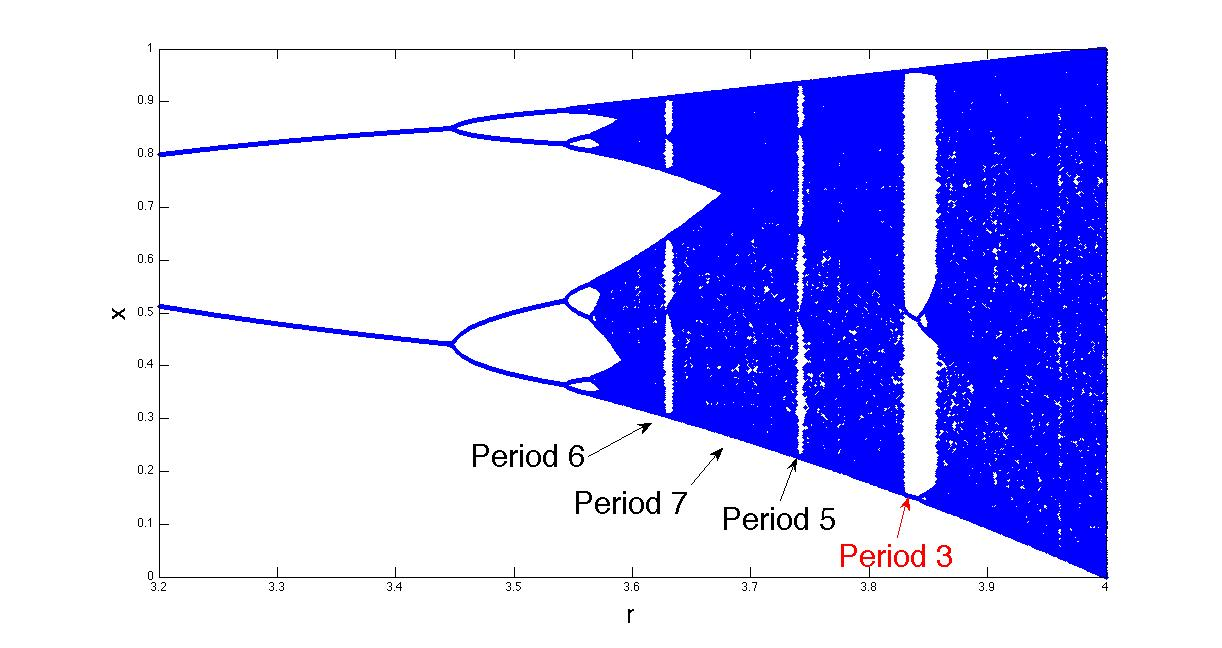
\includegraphics[height =3in, width = 5in]{logistic1.jpg}
%
%\end{frame}
%
%\begin{frame}
%\frametitle{Period 3 analysis}
%\vskip -1cm
%
%%\rightskip -2cm
%\begin{columns}
%
% \column{.6\textwidth}
%
%
%\begin{figure}[h!]
% 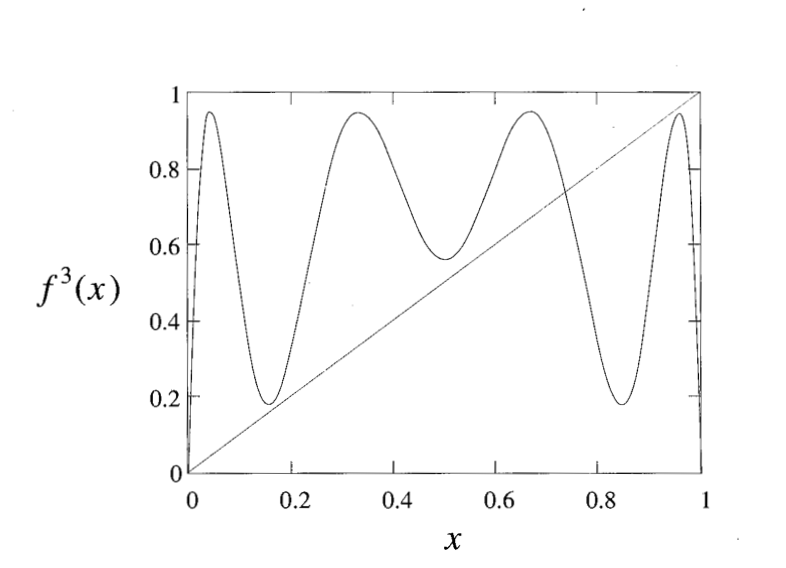
\includegraphics[height =2.1 in]{requals38} 
%
% \caption{ $r=3.8$} 
% \end{figure}
% \vskip .9cm
%\column{.5\textwidth}
%
%
%\begin{figure}[h!]
% 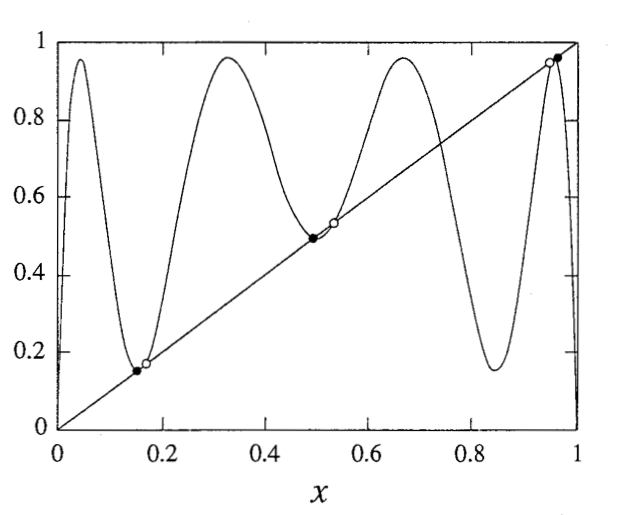
\includegraphics[height=1.91in]{requals3835}
% \caption{$r=3.835$\,\  {\scriptsize (See Strogatz) }}
% \end{figure}
%
%\end{columns}
%
%\end{frame}
%
%
%\begin{frame}
%\frametitle{Logistic map}
%\leftskip -1 cm
%%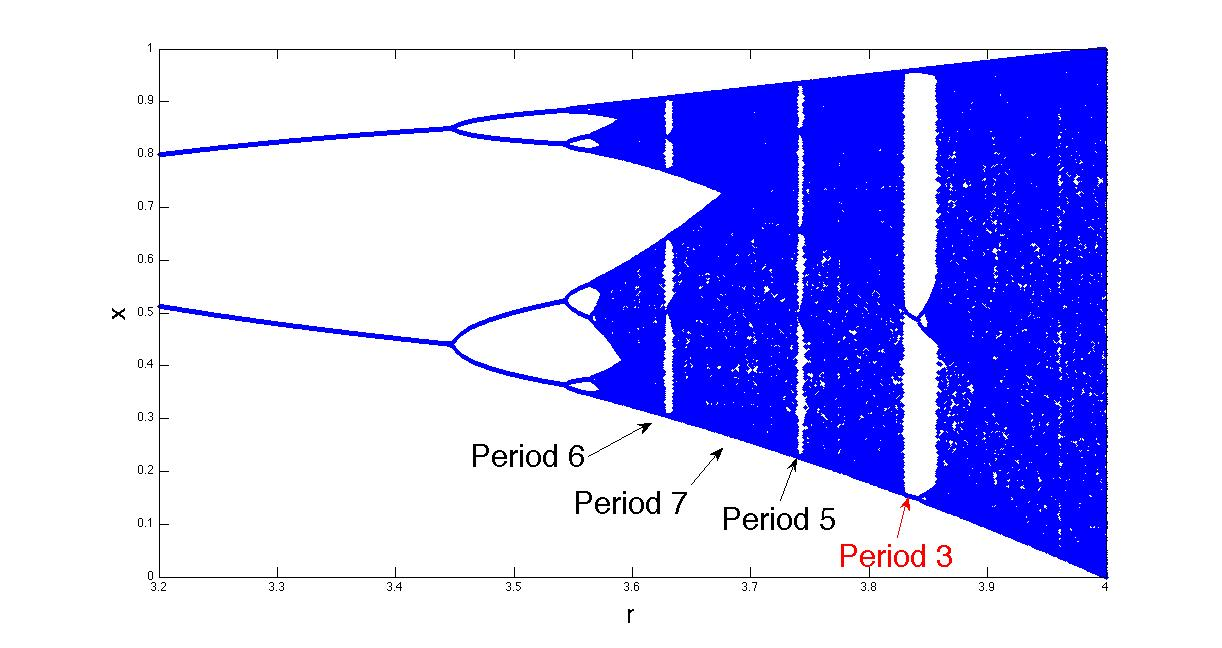
\includegraphics[height =1in]{logistic1.pdf}
%\begin{block}{Logistic map final remarks}
% \begin{itemize}
% \item As $r$ continuously increases from $0 \rightarrow 1 + \sqrt{8}$, periodic orbits of periods from bottom up in the Sarkovskii ordering gradually come into existence. 
%\item Before this $r$ value, there are NO period 3 cycles %yet this does not mean $F$ is not CHAOTIC for some of these prior $r$ values. 
% \item Having periods of arbitrary length is a hallmark of chaos, not a necessity, in our mathematical definition.
% \item Li and Yorke called a system "chaotic" if it had periodic points of arbitrary period length and an uncountable set of aperiodic points.
% \end{itemize}
%\end{block}
%\end{frame}
%
%\subsection[Other function types]{Counterexamples}
%\begin{frame}
%\frametitle{What if F is not 1-D continuous?}
%\begin{enumerate}
%\item Discontinuous Counterexample
%{\scriptsize
%\begin{columns}
%\column{.5\textwidth}
% \[ F(x) =  \begin{cases} x + \frac1 3 \,\,\, \mbox{if} \,\,0 \leq x < \frac 2 3\\
%x-\frac 2 3  \,\,\, \mbox{if} \,\, \frac 2 3 \leq x \leq 1
%\end{cases} \]
%It can be shown that every point on $[0,1)$ has period 3. ex. $\frac 1 6 \rightarrow \frac 1 2 \rightarrow \frac 5 6\rightarrow \frac 1 6$\\
%The value $x= 1$ is eventually period 3. \\
% No other periodic orbits exist for $F$.
%\column{.5\textwidth}
%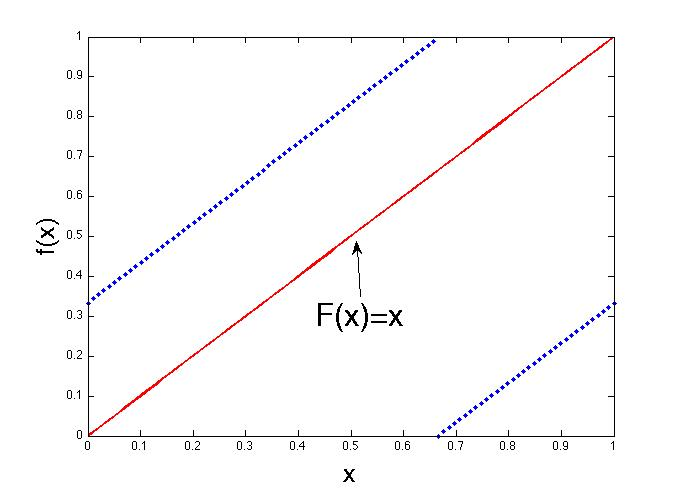
\includegraphics[height=4cm]{discont575.jpg}
%\end{columns}
%}
%
%\item Circle Map Counterexample
%\begin{itemize}
%{\scriptsize
%
%\item Theorem does not even hold on 1-D system that is not on real line. The map which rotates all points on a circle by $120^{\circ}$ makes all points periodic with period 3.
%}
%\end{itemize}
%%\item Glimmer of Hope
%%\begin{itemize}
%%{\scriptsize
%
%%\item Although to theorem does not have a higher-dimensional analogue, we can see typical behavior of period-doubling of cycles and period 3 windows in 3-D continuous time
%%systems like the R\"ossler system:
%%\begin{align*}
%%\dot{x} &= -y-z\\
%%\dot{y} &= x + ay\\
%%\dot{z} &= b + z(x-c) \,\,\,\,\,\, \mbox{see Strogatz for more detail}
%%\end{align*}
%
%%}
%%\end{itemize}
%
%\end{enumerate}
%\end{frame}
%
%\subsection[Summary]{Discussion Points}
%\begin{frame}
%\frametitle{Summary and Discussion points}
%
%{\scriptsize
%\begin{itemize}
%\item \emph{Glimmer of Hope:} Although to theorem does not have a higher-dimensional analogue, we can see typical behavior of period-doubling of cycles and period 3 windows in 3-D continuous time
%systems like the R\"ossler system:
%\begin{align*}
%\dot{x} &= -y-z\\
%\dot{y} &= x + ay\\
%\dot{z} &= b + z(x-c) \,\,\,\,\,\, \mbox{see Strogatz for more detail}
%\end{align*} 
%\item Possibilities in twist maps (see Laskar et al.) and other higher dimensional systems.
%\item An elegant result about existence of orbits in 1-D maps with ONLY the assumption that $F$ is continuous!
%\end{itemize}
%}
%\begin{block}{Herman Melville, \emph{Moby Dick}}
%\centering
%"The classification of the constituents of a \emph{chaos}, nothing less here is essayed.``
%\end{block} 
%\end{frame}
%\begin{frame}
%\centering
%\shadowbox{\Huge {THANK YOU!}}\\
%
%References:\\
%{\scriptsize
%\begin{thebibliography}{4}
%
%\bibitem{Devaney}
%Devaney, R. L. (2003). An Introduction to Dynamical Systems 2nd ed.  . {\sl Advanced Book Program}.
%
%\bibitem{Gleick}
%Gleick, J. (1987). Chaos: Making a New Science {\sl Penguin Books}
%
%\bibitem{Li} Li, T., Yorke, J. A.  (1975).  Period Three Implies Chaos.  {\sl The American Mathematical Monthly}, {\bf v 82}, 985-992.
%
%\bibitem{May}
%May, R. M. (1976). Simple mathematical models with very complicated dynamics. {\sl Nature}, {\bf v 261}, 459-467.
%
%\bibitem{Strogatz}
%Strogatz, S.H. (1994) Nonlinear Dynamics and Chaos. {\sl Da Capo Press}
%
%\end{thebibliography}
%}
%\centering
%For your hardcore listening pleasure, check out:\\
%\begin{columns}
%\column{.5\textwidth}
%\centering
%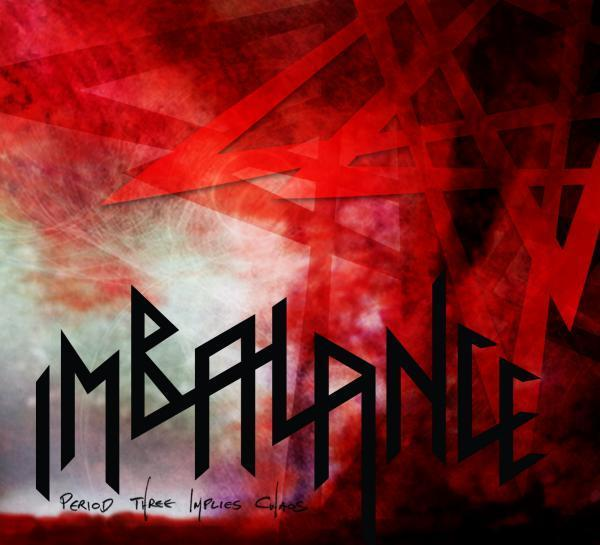
\includegraphics[height=2 cm]{imbalance.jpg}
%\column{.5 \textwidth}
%\emph{Period Three Implies Chaos} \\
%by: IMBALANCE
%
%\end{columns}
%\end{frame}

\end{document}
